\section{Actividad 12}

\subsection*{Se tiene una señal 
$
m_1(t) = A_{m1}\cos(2\pi f_{m1}t)
$
y una señal 
$
m_2(t) = A_{m2}\cos(2\pi f_{m2}t)
$
que se aplican a los canales izquierdo y derecho respectivamente, 
de un generador de señal modulante para FM estéreo.  
Si $m_1(t)$ es de $2~V_{pp}$ y $f_{m1} = 5.2~\text{kHz}$, mientras que 
$m_2(t)$ es de $3~V_{pp}$ y $f_{m2} = 6~\text{kHz}$, graficar la respuesta en frecuencia 
de la señal $m(t)$ que modulará a una portadora de $101.7~\text{MHz}$ 
de un transmisor de FM estéreo.}


Se tienen las siguientes señales:

\begin{itemize}
    \item $m_1(t) = cos(2\pi 5200t)$
    \item $m_2(t) = 1.5cos(2\pi 6000t)$
\end{itemize}

La señal multiplexada esta dada por:
    \[
        m(t) = [m_1(t) + m_2(t)] + [m_1(t) - m_2(t)] \cos(4 \pi f_c t) + k\cos(2 \pi f_c t) 
    \]
donde $f_c=19~[kHz]$ y K es la amplitud del tono piloto.\par

Reemplazando los datos en la  señal multiplexada se obtiene:

    \[
        m(t) = [cos(2\pi 5200t) + 1.5cos(2\pi 6000t)] + [cos(2\pi 5200t) 
    \]
    \[
     - 1.5cos(2\pi 6000t)] \cos(4 \pi 190000 t) + k\cos(2 \pi 19000 t) 
    \]
Distribuyendo el $\cos(4 \pi 190000 t)$ se tiene que:
    \[
        m(t) = cos(2\pi 5200t) + 1.5cos(2\pi 6000t) + cos(2\pi 5200t)\cos(4 \pi 190000 t)
    \]
    \[
        - 1.5cos(2\pi 6000t)\cos(4 \pi 190000 t) + k\cos(2 \pi 19000 t) 
    \]
Utilizando la identidad trigonométrica $\cos(\omega_1)\cos(\omega_2) = \frac{1}{2}[\cos(\omega_1 + \omega_2) + \cos(\omega_1 - \omega_2)]$ y que $\cos(4\pi 19000t) = \cos(2\pi 38000t)$, se obtiene que $m(t)$ es:

    \[
        m(t) = \cos(2\pi 5200t) + 1.5\cos(2\pi 6000t) + \frac{1}{2}\cos[2\pi (5200 + 38000)t] 
    \]
    \[
        + \frac{1}{2}\cos[2\pi (5200 - 38000)t] - \frac{1.5}{2}\cos[2\pi (6000 + 38000)t] + \frac{1.5}{2}\cos[2\pi (6000 - 38000)t]
    \]
    \[
         + k\cos(2\pi 19000t)
    \]
    \[
        = \cos(2\pi 5200t) + \frac{3}{2}\cos(2\pi 6000t) + \frac{1}{2}\cos(2\pi 43200t) + \frac{1}{2}\cos(2\pi (-32800)t)
    \]
    \[
        - \frac{3}{4}\cos(2\pi 44000t) - \frac{3}{4}\cos(2\pi (-32000)t) + k\cos(2\pi 19000t)
    \]

Aplicando la transformada de Fourier a la señal $m(t)$ se obtiene que:

    \[
        M(f) = \frac{1}{2}[\delta(f - 5200) + \delta(f + 5200)] + \frac{3}{4}[\delta(f - 6000) + \delta(f + 6000)] 
    \]
    \[
        + \frac{1}{4}[\delta(f - 43200) + \delta(f + 43200)] + \frac{1}{4}[\delta(f - (-32800))
    \]
    \[
         + \delta(f + (-32800))] - \frac{3}{8}[\delta(f - 44000) + \delta(f + 44000)]
    \]
    \[
        - \frac{3}{8}[\delta(f - (-32000)) + \delta(f + (-32000))] 
    \]
    \[
     + \frac{k}{2}[\delta(f - 19000) + \delta(f + 19000)]
    \]

En la Figura \ref{fig:espectro_ej12} se muestra el espectro de la señal m(t).

    \begin{figure}[H]
        \centering
        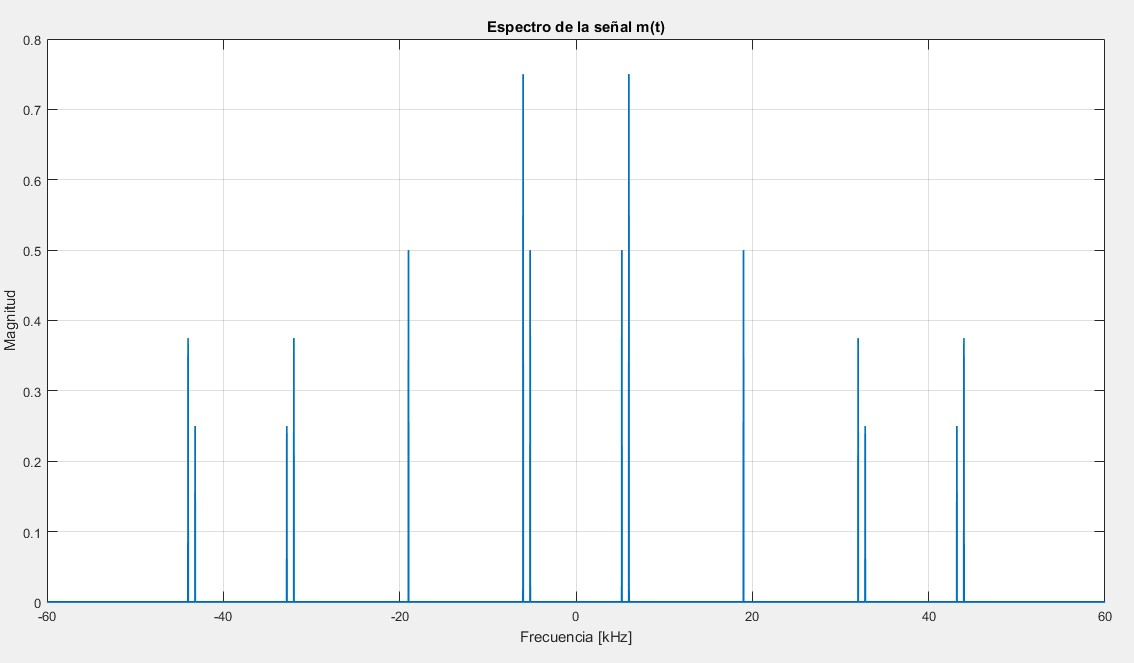
\includegraphics[width=0.8\linewidth]{imagenes/Parte_2/Actividad_12/ejercicio_12.jpg}
        \caption{Espectro de la señal m(t).}
        \label{fig:espectro_ej12}
    \end{figure}